\section{Design}
\label{s:ch5-Design}
Before diving into implementing the code, it is always imperative to have a
whiteboard and design the architecture of the tool being built. The tool that
will be made will have a single source of truth for a schema that will then be
taken and processed through the logic of the application and transformed into
structured folders containing files that represent each living part of the
source. The markdown will support framework-agnostic plug-in and integration,
meaning that any JSX framework can parse it and build HTML static files that any
browser can read. It is vital to support as many types and Scalars as possible
to consistently generate the files from any schema, regarding their complex tree
structure and the scalars used by the producer. The diagram below visually
explores the solution that will be chased for the end goal.

\begin{figure}[H]
  \centering
  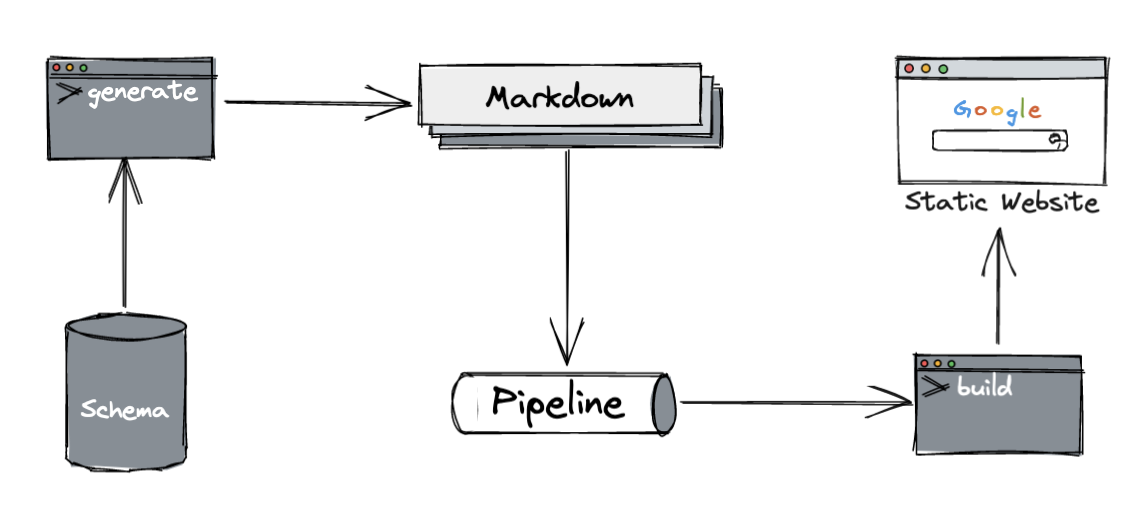
\includegraphics[width=0.7\textwidth]{figures/architecture}
  \caption{High-Level Architecture}
  \label{f:ch5-architecture}
\end{figure}

\section{Proof of Concept}
\label{s:Proof of Concept}
This section will discuss the first iteration of the project as Proof of Concept
(PoC). This will be the initial implementation stage of the project used for
discovery and testing. The PoC is a software development methodology that helps
the project developers implement the initial logic and validate their hypothesis
on the project's feasibility. This specific PoC will be coded in JavaScript
using Node as a backend runtime. In a perfect world, the tool should be written
using a more robust programming language and ecosystem such as Scala to have the
advantage of an effectful, high-performance in pure functional programming. This
would massively improve concurrency with the use of IO, which facilitates Fibers
as a replacement for native OS threads and allows for the benefit of millions of
concurrent processes without the need for a thread manager. In this use case,
the PoC is using JavaScript to keep things simple, without looking too much at
the performances that it would have in a production environment as it will be
only used to demonstrate how feasible the project is. Since JavaScript does not
support the concept of template literals, a templating language named Handlebars
will be used to generate the inside structure of the markdown files. Handlebars
use expressions that are evaluated and replaced with the evaluation results. An
example of this can be seen below.

\begin{figure}[H]
  \centering
  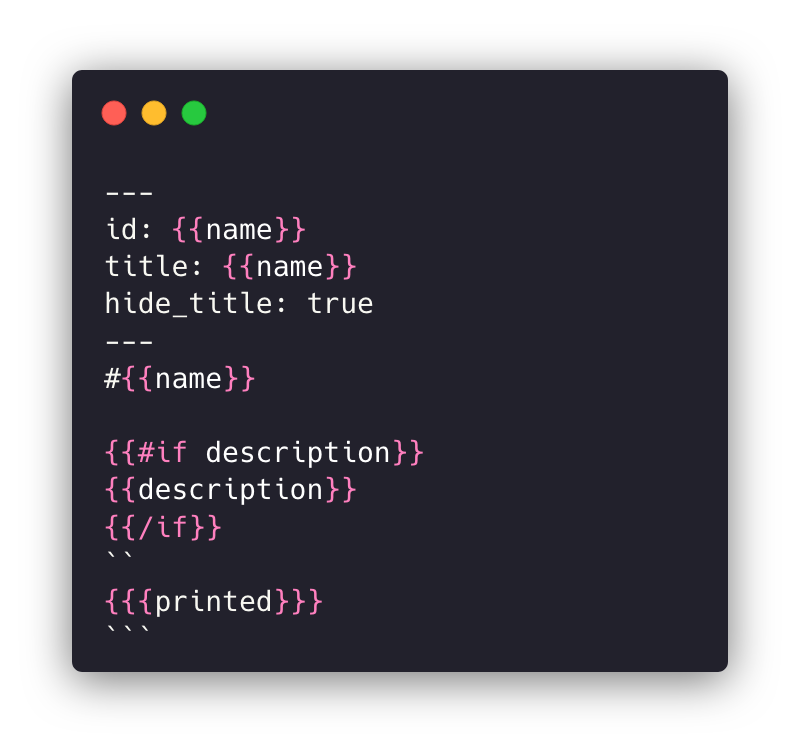
\includegraphics[width=0.5\textwidth]{figures/code/handlebars.png}
  \caption{Handlebars Template Language}
  \label{f:ch5-handlebars-template-language}
\end{figure}

The imports for the PoC will be kept at the very minimal. Below is shown
the start of the index file with the imported tools to complete and reach the
end goal.
\
\begin{figure}[H]
  \centering
  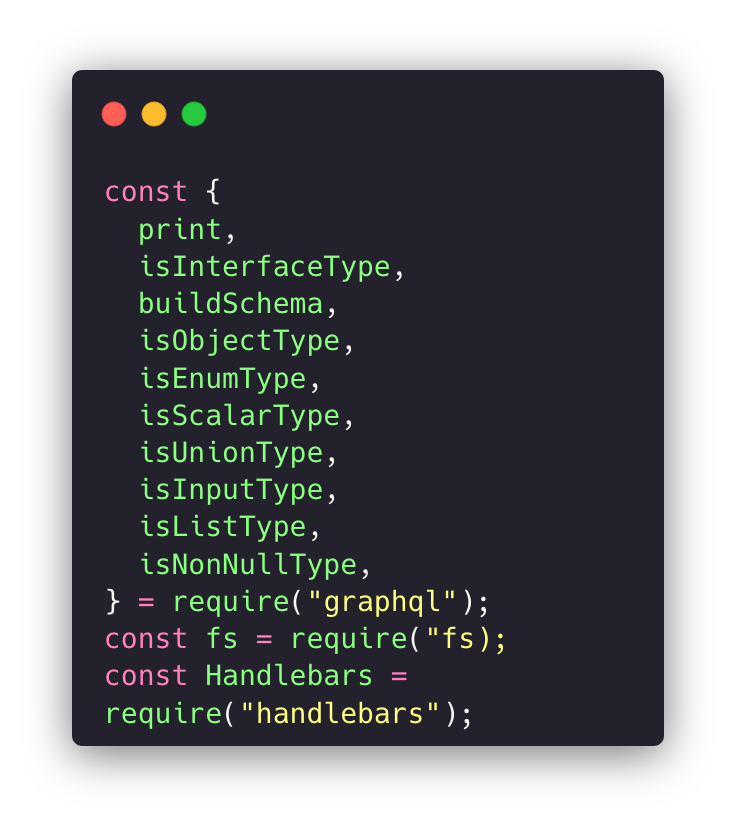
\includegraphics[width=0.5\textwidth]{figures/code/poc-imports.png}
  \caption{PoC Imports}
  \label{f:ch5-poc-imports}
\end{figure}

In order for it to work, we need to install the GraphQL library and import
all the type guards that are implemented in it to be able to check the types
while navigating in the complex nested structure of the Abstract Syntax Tree (AST)
generated by the reading the schema given in the folder. An example on how the
type guards are implemented is shown in the image below.

\begin{figure}[H]
  \centering
  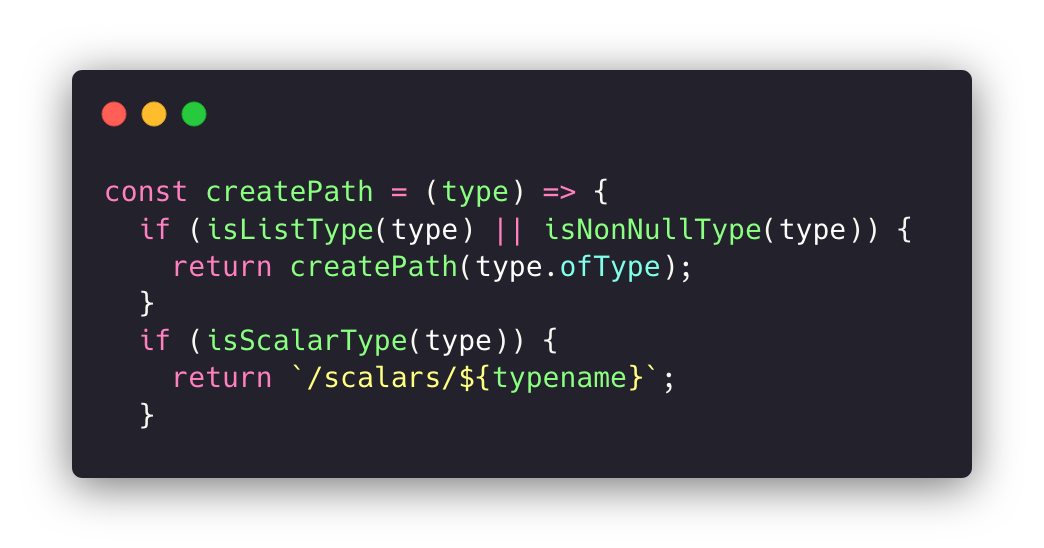
\includegraphics[width=0.5\textwidth]{figures/code/poc-type-guards.png}
  \caption{PoC Type Guards}
  \label{f:ch5-poc-type-guards}
\end{figure}

Since in the markdown file, there are places where it would be nice to have
hyperlinks that point the user to the right page when navigating the
relationship between the fields, there is a need of the type guards to be able
to place the right path into the object of a specific formatted data structure
used to group the data. An example of the object related to the image above is
shown below.

\begin{figure}[H]
  \centering
  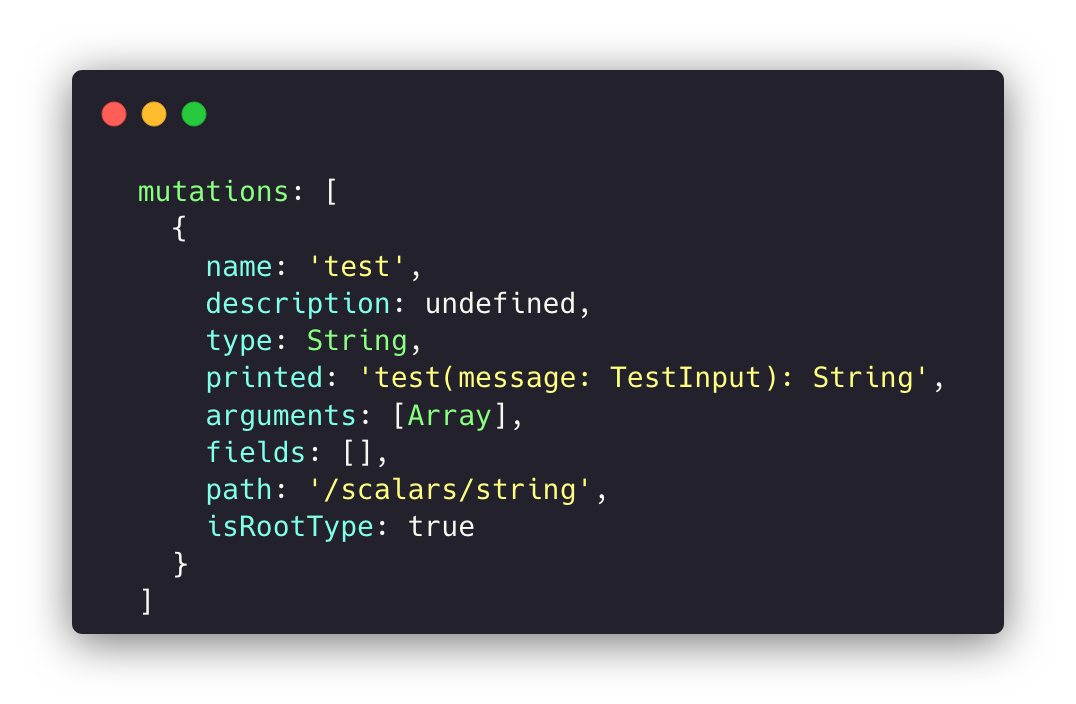
\includegraphics[width=0.5\textwidth]{figures/code/poc-scalar-type.png}
  \caption{PoC Scalar Path}
  \label{f:ch5-poc-scalar-path}
\end{figure}

As shown in the image above, the field has a type of \texttt{String} and the
path to the scalar is \texttt{/scalar/string}. The type guard is implemented as
a way to recursively navigate the AST and find the right path to the each
specific hyperlink case.

\begin{figure}[H]
  \centering
  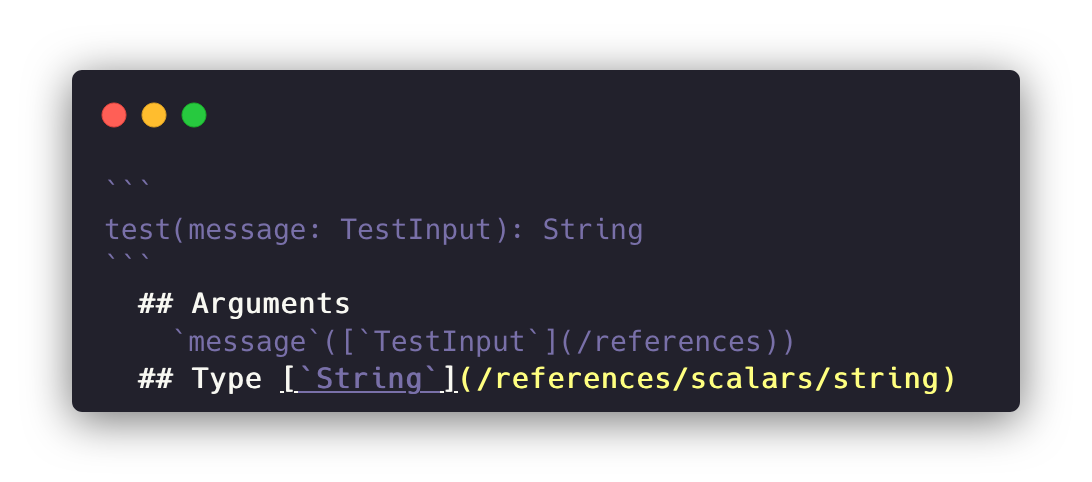
\includegraphics[width=0.5\textwidth]{figures/code/poc-generated-path.png}
  \caption{PoC Scalar Path Markdown}
  \label{f:ch5-poc-scalar-path-markdown}
\end{figure}

The image above shows the exact same mutation but in a generated markdown format,
completely done by the tool.

In order to have a great structure of the data we are going to manipulate for
the generation, a special lambda function has been created which return an object
with all the properties each type has to offer, it goes and traverse the AST and
places the information in the right properties available for later use.

\begin{figure}[H]
  \centering
  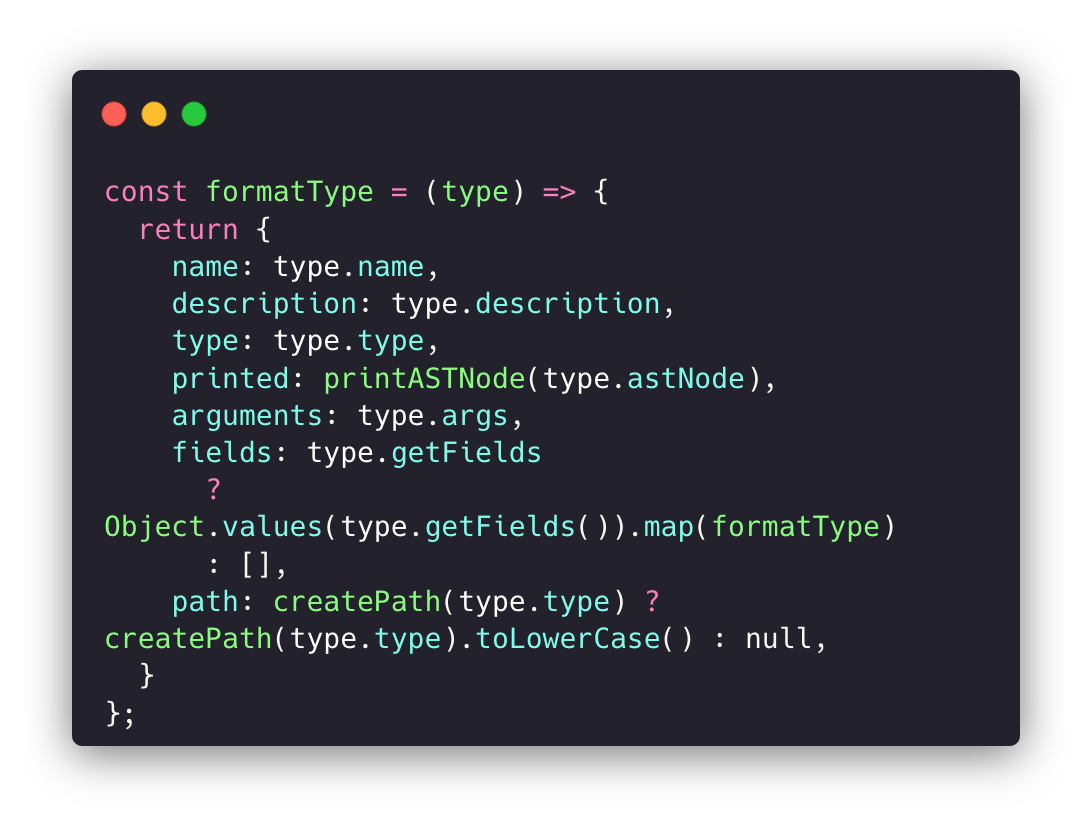
\includegraphics[width=0.5\textwidth]{figures/code/poc-format-type.png}
  \caption{PoC Format Type Lambda Function}
  \label{f:ch5-poc-format-type-lambda-function}
\end{figure}

It is important to note there is another function operating in the body formatType
which is used to pull out the printed version taken from the schema. This is
useful to have so that the documentation can have an original representation of
the piece of schema that is being discussed. The image below represent the function
written to achieve the printed version of the schema in the formatted structure.

\begin{figure}[H]
  \centering
  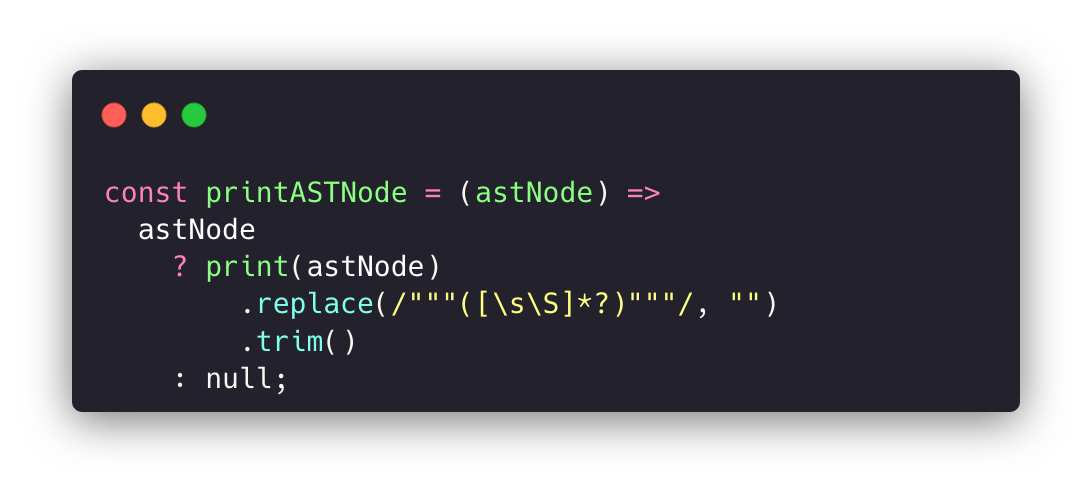
\includegraphics[width=0.5\textwidth]{figures/code/poc-print-ast.png}
  \caption{PoC Print AST Node}
  \label{f:ch5-poc-print-ast-node}
\end{figure}

It is again a lambda function that is used to traverse the AST till it reaches a
specific node and then surgically extract the printed version of it, making sure
it doesn't have any unwanted literal strings, characters or whitespace in it, so
that it can directly be used without any further manipulation in the templating
system previously described.

One of the last pieces of the puzzle is a wrapper that groups all types in a
last and single object, done used the previously described functions recursively
for any type in the AST. This prints out a massive object that is then used in a
nested loop to again recursively generate the markdown files for each type, while
accessing the Handlebars templating for valuating the expressions.

The structure of the final, but empty, data structure is as shown below.


\begin{figure}[H]
  \centering
  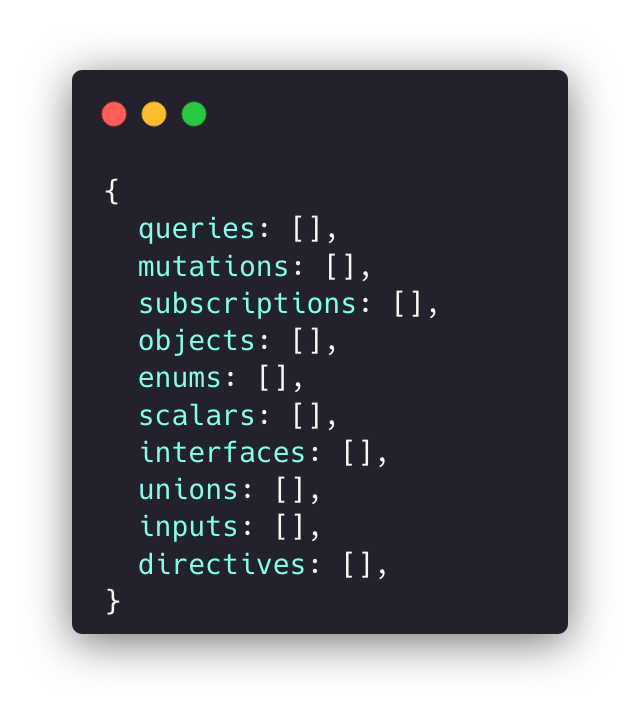
\includegraphics[width=0.5\textwidth]{figures/code/poc-empty-structure.png}
  \caption{PoC Empty Structure}
  \label{f:ch5-poc-empty-structure}
\end{figure}

The structure is being shown as empty because it would be too much to show in a
single image. In order to facilitate the understanding, below also an image
representing a single type with its full array structure.

\begin{figure}[H]
  \centering
  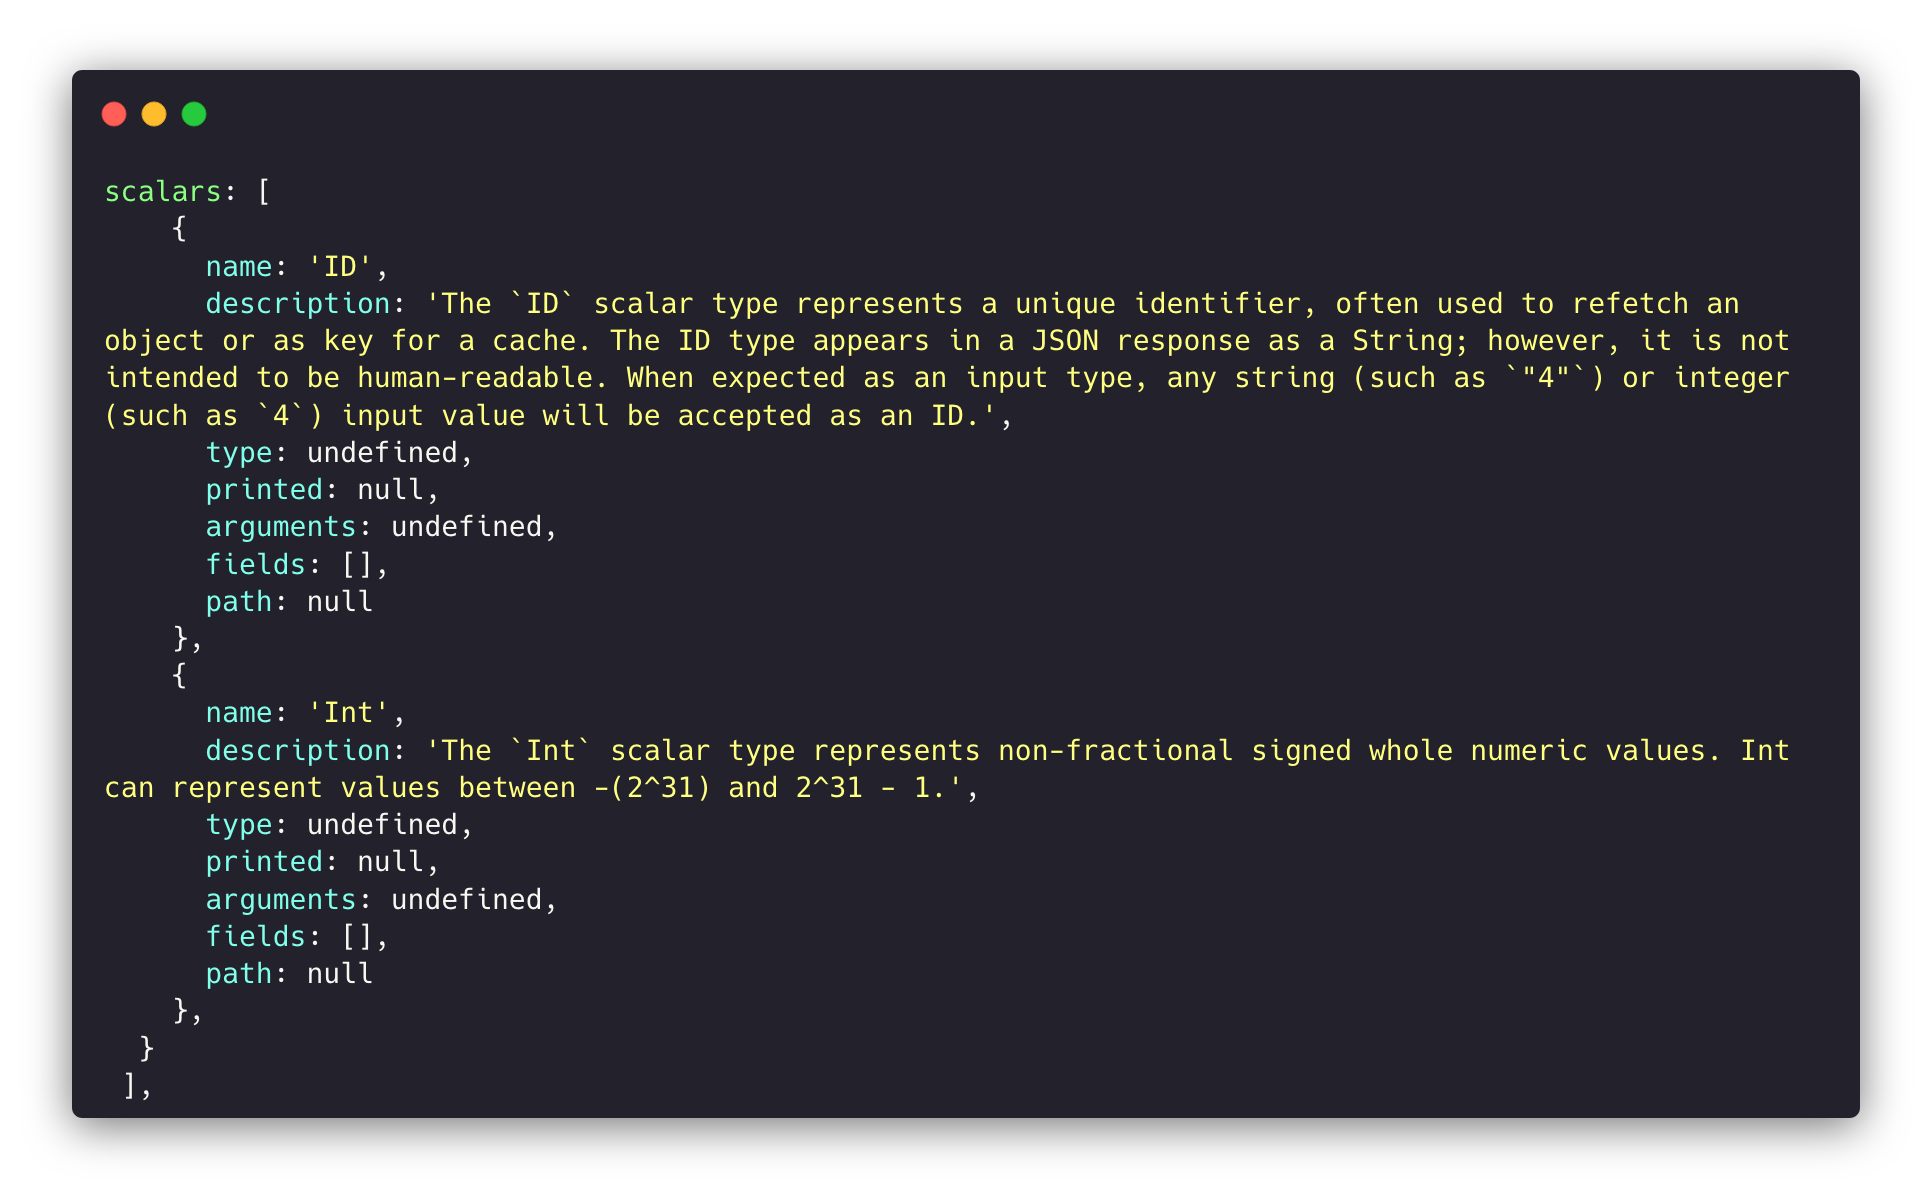
\includegraphics[width=0.8\textwidth]{figures/code/poc-full-structure.png}
  \caption{PoC Full Structure}
  \label{f:ch5-poc-full-structure}
\end{figure}

And as previosuly mentioned, the final structure is then used in a nested
function shown below.

\begin{figure}[H]
  \centering
  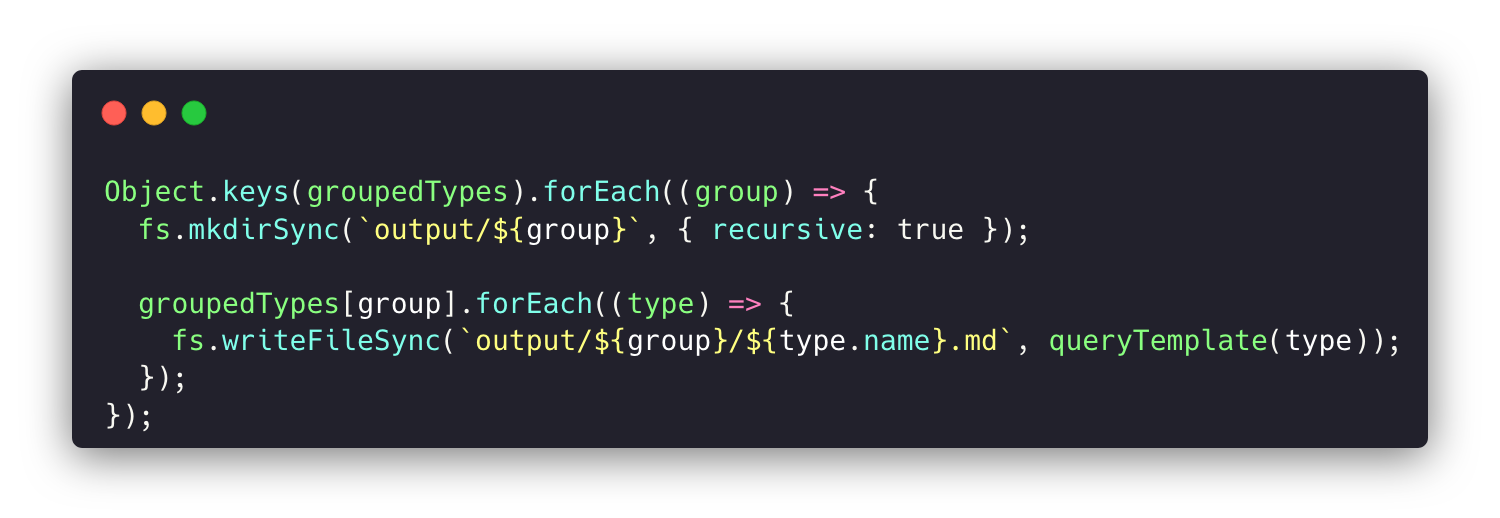
\includegraphics[width=0.8\textwidth]{figures/code/poc-nested-function.png}
  \caption{PoC Nested Loop}
  \label{f:ch5-poc-nested-loop}
\end{figure}

The nested loop makes sure that all the types are accounted for and uses the
templating system to generate the markdown files for each type.

The final output is an output folder with all the markdown files generated, and
the goal of the PoC has been validated and the code is ready to be used and
refactored for better improvements and use cases.

\begin{figure}[H]
  \centering
  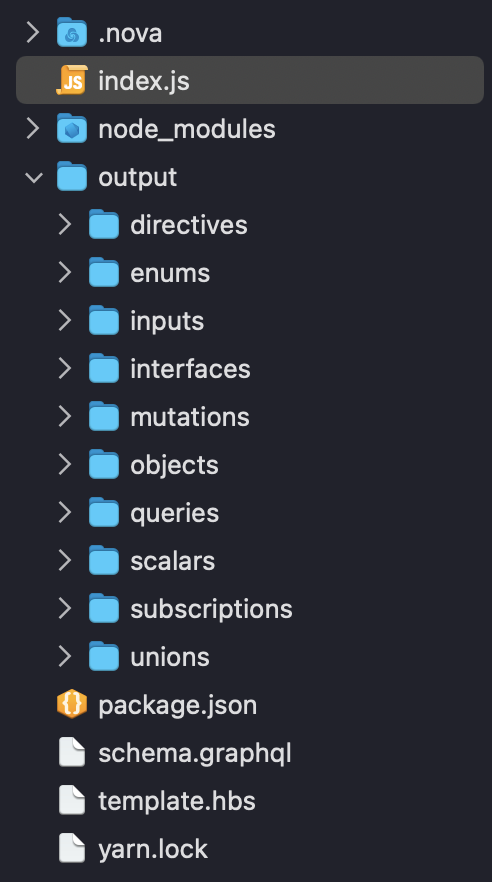
\includegraphics[width=0.3\textwidth]{figures/folders}
  \caption{PoC Output Folder}
  \label{f:ch5-poc-output-folder}
\end{figure}

Each folder has multiple md files that can be used by any framework that can
parse the markdown files and build static generated pages in HTML.

Now that the proof of concept has been completed and resulted in a successfull
experiment, the next step is to refactor the code and removing unnecessary steps
such as Handlebars templating, which will be redundant with TypeScript. It is
always good to keep the dependencies as minimum as possible in order to keep the
code clean and easy to maintain. Easy to maintain because deprecation of
functionalities are always behind the corner and it means that the code needs to
be migrated to a new version of the library which would require time, effort and
money.

\section{Refactoring}
\label{s:Refactoring}
For the same reasons explained before, the code will be then refactored in
TypeScript removes the templating system and utilises the one in-built with the
language. The template literals types will produce the same result shown and
achieved in the JavaScript PoC, making it much more succinct, readable and
powerful as the code will not be decoupled in different files and folders. It
will also keep the code much more DRY with a single source of truth, which the
language itself tries to doctrine. The main reasons to migrate any project from
JavaScript to TypeScript are listed below.

\subsection{TypeScript Module Support}
\label{ss:TypeScript-Module-Support}
TypeScript supports modules, meaning that any classes, variables and functions
can be exported and imported in other files using the keywords provided by the
default API similarly to what is done in ECMAScript 2015. Any file containing
import and export keywords will be considered as a module, and those without
top-level declarations are considered scripts available globally. A perfect
example can be seen in one of the types that are being exported in the
refactored tool, in the image below.

\begin{figure}[H]
  \centering
  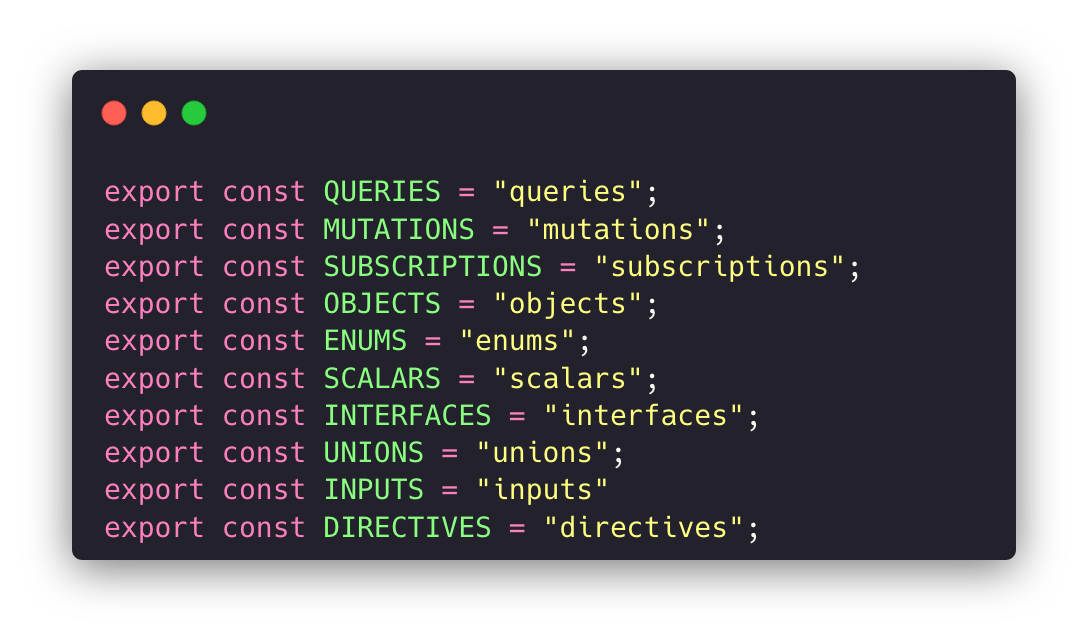
\includegraphics[width=0.5\textwidth]{figures/code/constants.png}
  \caption{Constants File}
  \label{f:ch5-refactored-constants-and-types}
\end{figure}

This file contains a set of strings used as keys in the larger object containing
all the types and their formatted data. It is very convenient to have a bunch of
constants and not have the names of the keys hardcoded directly in the object
for both readability and convenience in case of later refactoring.

\subsection{TypeScript Class Support}
\label{ss:TypeScript-Class-Support}
TypeScript is a superset of JavaScript, or even better an object oriented
version of JavaScript. Even though TypeScript is considered object oriented
programming, it also has and shares many common features with function
programming languages. A class in TypeScript is a recipe to create objects, very
similarly to any other object oriented programming languages that have also been
covered at the University. This feature could be a very huge selling point to
any developer used to Java as main backend language, so that it will be easy to
switch from one language to another in case the company has two different
languages in different codebases. In this project, there is a slightly different
approach as a class has not been used and the methodology leans more towards
a functional programming approach without the use of any functional programming
libraries such as Lodash or fp-ts, to keep everything as simple as possible.

\subsection{TypeScript Type Support}
\label{ss:TypeScript-Type-Support}
This is the main reason why TypeScript is a better choice than JavaScript, the
type system. TypeScript is statically typed, maening that all checks are done
at compile time, and not at runtime. The compiler will throw an error if variables
and expressions do not match the type that is expected. This is all out of the box,
for free, and right into any IDE of choice.
The primitive types that TypeScript supports are: strings, boolean and numbers.
On top of that, it also support a very special type called Union, which is a way
to combined and build new types out of already defined or in-built types.

\begin{figure}[H]
  \centering
  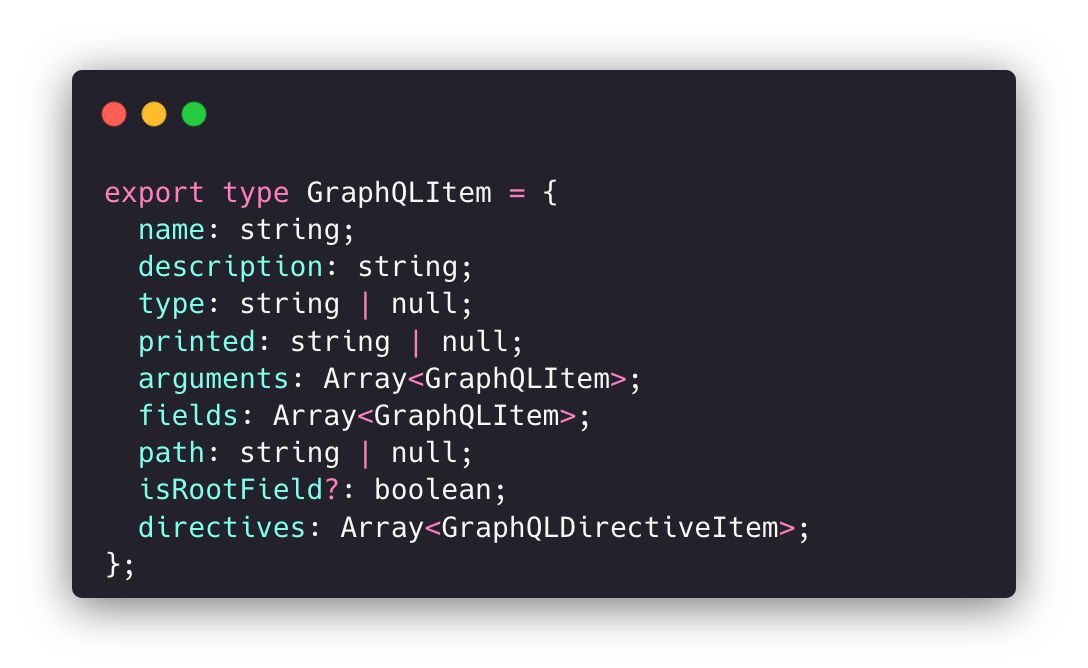
\includegraphics[width=0.5\textwidth]{figures/code/union-types.png}
  \caption{Union Types}
  \label{f:ch5-refactored-union-types}
\end{figure}

In the image above, the Union type is used to combine some primitives such as
string with a nullable type which is a special type which make the whole type
nullable. Nulls and undefined are the two special types of TypeScript and are
very annoying to deal with. Even their creator, Tony Hoare, realised it and
admitted it was one of his biggest professional mistakes, or more specifically,
his ``billion dollar mistake''. The GraphQLItem type shown in the image above,
is a representation of the formatted object we previously used to represent data
in the proof of concept section. Creating such a type is very simple and
effective, meaning any value that the object takes, will need to adhere with the
strict type rules provided, and nothing less. If the manipulation of data would
result in a differenty kind of primitives or newly created type to be used and
filled in the object, it will instantly be shown as an error in the IDE and will
not compile.

\subsection{TSConfig}
\label{ss:TSConfig}
To be able to use TypeScript in the project, it needs to be installed with
\texttt{yarn install -d typescript}. It will add TypeScript to the
\texttt{package.json}. Other packages like \texttt{ts-node, jest, eslint}
needs to be installed for the project to compile and run. It will also add
support for tests which will be shown in later chapters.
On top of that, a new file named \texttt{tsconfig.json} needs to be created at the
root of the TypeScript project which specified the root files and the options
given to the compiler for when its time to compile. The options given in this
project are the following listed in the image below, which is taken from the
project itself.

\begin{figure}[H]
  \centering
  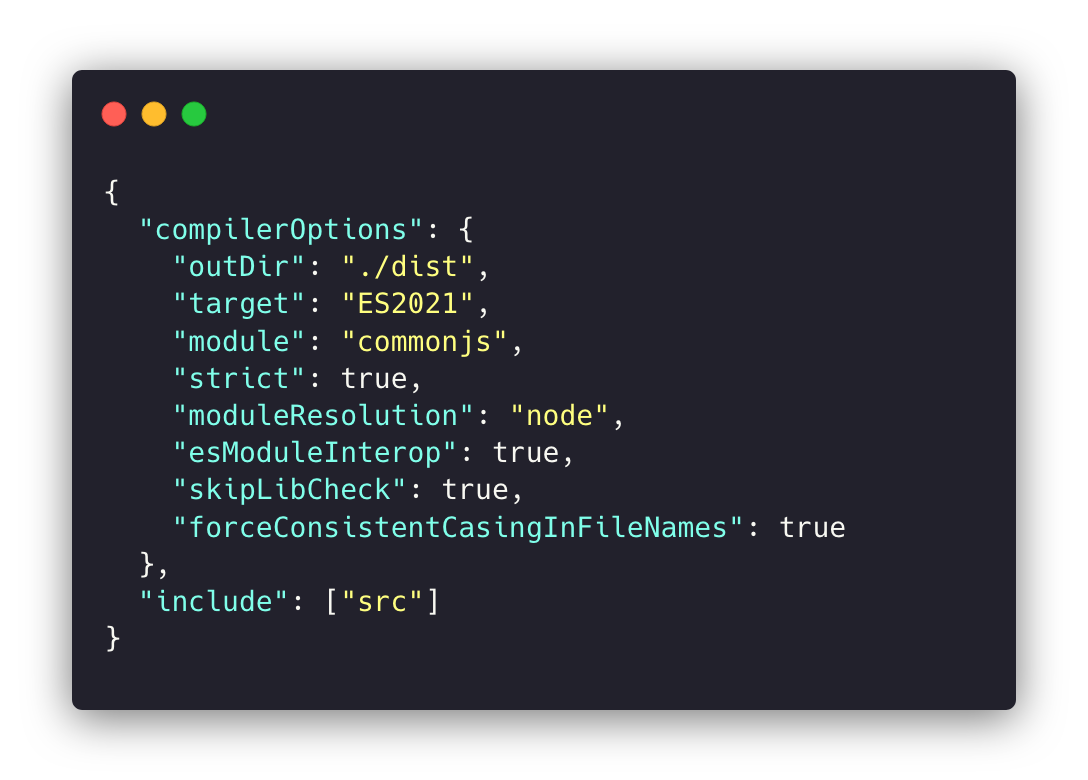
\includegraphics[width=0.5\textwidth]{figures/code/tsconfig.png}
  \caption{TSConfig}
  \label{f:ch5-refactored-tsconfig}
\end{figure}

The root object starts with \texttt{compilerOptions} which is an object itself
that contains the options the compiler will read to compile and build the project.
The \texttt{outDir} option is used to direct the files on a specific folder when
the command \texttt{tsc} is given to build the project. It will take the
TypeScript files, and convert them in JavaScript files in the destination folder
which will look something like the folder structure shown in the picture below.

\begin{figure}[H]
  \centering
  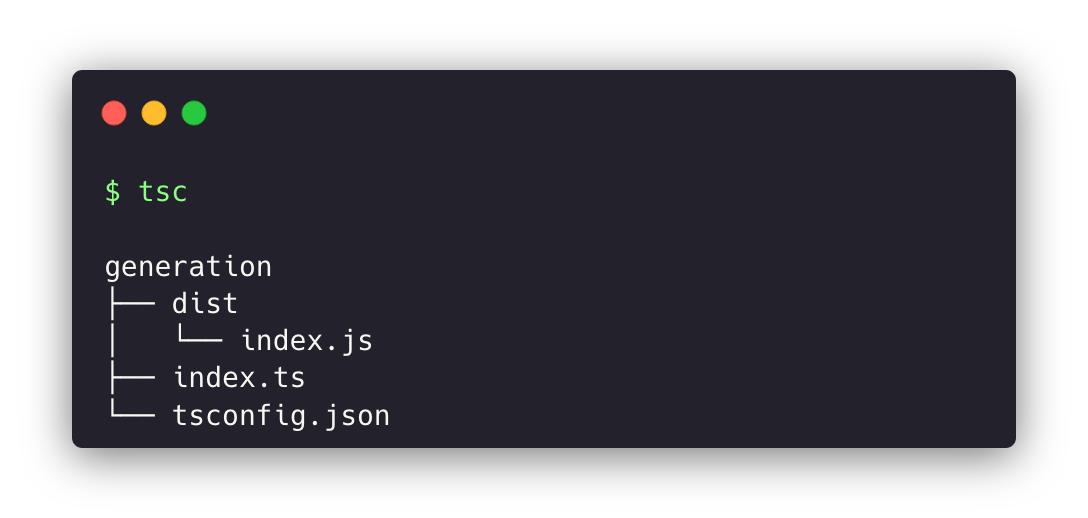
\includegraphics[width=0.5\textwidth]{figures/code/outdir.png}
  \caption{OutDir Option Result}
  \label{f:ch5-refactored-outdir}
\end{figure}

The module option is to specify the module system that will be used in the
project.The \texttt{target} option is used to specify the target version of
JavaScript will be produced from a given piece of TypeScript code. In this case
the project will use the most up to date version of ECMAScript (ES).The option
\texttt{strict} is the most important and also interesting one as it is a little
shortcut to enable many strict rules options, to be more specific seven, which
they all make the code to have much more strict rules on type checking, which
will be very good as stricter is synonym of better and safer. The seven options
included in the strict shortcut are the following: \texttt{noImplicitAny},
\texttt{noImplicitThis}, \texttt{alwaysStrict}, \texttt{strictBindCallApply},
\texttt{strictNullChecks}, \texttt{strictFunctionTypes}, and
\texttt{strictPropertyInitialization}.

\newpage
Below a deep explaination of the options being used in this project:
\begin{itemize}
  \item \texttt{noImplicitAny}: is probably the most important as it basically
  forces the developers to the usage of TypeScript and won't allow JavaScript at
  all costs. Any code written in JavaScript, for example omitting the type in a
  parameter of a function, will return an error in the compiler and the IDE
  itself. This is because, if no type is assigned, it will implicitly be
  assigned to a type called any, hence the name of the option. It is not good
  practice, but it is still possible to explicitly assign the any type to any
  variable or parameters and make the compiler not complain about it.
  \item \texttt{noImplicitThis}: is another option that is used to prevent
  implicit this usage in TypeScript. This is a very good option to use as it
  will prevent implicit this usage in TypeScript and will return an error in the
  compiler and the IDE itself.
  \item \texttt{alwaysStrict}: is used to imaginary place a \texttt{"use
  strict"} statement on top of any and every compiled JavaScript file that will
  be generated from TypeScript.
  \item \texttt{strictBindCallApply}: is used to prevent a common loophole
  that would make the type check not working in certain situations. This
  certainly is not a good thing, so keeping this option enabled is reccomended
  in any project.
  \item \texttt{strictNullChecks}: is a good option to prevent variables
  with inferred or explicitly types to be assigned as null or undefined.
  \item \texttt{strictFunctionTypes}: is an option that could be a little
  intimidating to explore and understand as it cover the world covariance and
  contravariance, which are topics that are covered more in programming
  languages such as Scala and are mostly used to build libraries as they are
  quite advanced. For the purpose of this explaination, this option force the
  function type parameter checks to be contravariant instead of bivariant and it
  applies to all function types with the exception of the those that comes from
  constructors and methods declaration.
  \item \texttt{strictPropertyInitialization}: this is related to classes and
  a member of a class needs to be initialised with a value in the declaration or
  constructor, otherwise an error will be thrown.
\end{itemize}

\subsection{Packet Manager}
\label{ss:Packet-Manager}

A package manager js used to manage any project dependencies in different ways.
It allows the developers to execute operations such as deleting, updating or
installing packages or running scripts. NPM stands for Node Package Manager, and
it was created in 2010. NPM is composed of three main parts: a website for user
experience regarding npm aspects, a registry where all the packages are
installed and released for the user, and a CLI to perform an operation from the
terminal. Yarn was created in 2016, and it immediately showed more extraordinary
performance than npm. It allowed the creation of a .lock file that contained the
list of the version installed for each dependency, allowing repository sharing
improvements. The main difference between these two package managers is how they
run operations. In fact, Yarn uses a parallel way by installing decencies at the
same time while NPM installs one package at a time. This increases performance
and speed on any kind of operation for the dependencies and is the main reason
why Yarn is the preferred package manager in this project, but also in the rest
of the world.

\section{Frontend}
\label{s:Frontend}
In this part I will show how I produced the frontend part that generates the
website.

\section{Version Control System}
\label{s:Version-Control-System}
GitHub etc

